\documentclass[11pt,a4paper]{article}
\usepackage[margin=2.5cm]{geometry}
\usepackage{amsmath,amssymb,amsthm}
\usepackage{hyperref}
\usepackage{xcolor}
\usepackage{listings}
\usepackage{graphicx}
\usepackage{tikz}
\usetikzlibrary{arrows.meta,positioning,shapes,calc}
\usepackage{booktabs}
\usepackage{enumitem}
\usepackage{mdframed}

\definecolor{cyan}{RGB}{68,221,255}
\definecolor{orange}{RGB}{255,136,68}
\definecolor{yellow}{RGB}{255,221,68}
\definecolor{pink}{RGB}{255,68,170}
\definecolor{green}{RGB}{68,255,136}
\definecolor{purple}{RGB}{170,68,255}
\definecolor{codebg}{RGB}{30,30,40}

\hypersetup{colorlinks=true,linkcolor=blue,urlcolor=blue}

\title{\textbf{cubical-viz: Phase 3 Feature Design}\\
\large Five Advanced Visualization Features}
\author{Oguri Cap}
\date{March 2026}

\begin{document}
\maketitle
\tableofcontents
\newpage

% ─────────────────────────────────────────────────────────────────────────────
\section{Overview}

This document describes the detailed visual and interaction design for five
advanced features planned for \texttt{cubical-viz}, a browser-based interactive
visualizer for cubical type theory. These features go beyond the individual rule
illustrations completed in Phase~1 and~2 and address higher-level pedagogical
goals: showing the structure of proofs, relating rules to one another, and
guiding the user through complete constructions.

\medskip
\noindent\textbf{Features covered:}
\begin{enumerate}
  \item Proof Relevance Panel
  \item Higher-Dimensional Paths (Square and Cube as Typed Terms)
  \item The Face Lattice $\mathbb{F}$
  \item Univalence Proof Walkthrough
  \item Dependency Graph Navigation
\end{enumerate}

\medskip
\noindent Each section follows the same structure: motivation, typing rule(s),
3D visualization design, step breakdown, interaction model, and implementation
notes.

% ─────────────────────────────────────────────────────────────────────────────
\section{Proof Relevance Panel}

\subsection{Motivation}

In cubical type theory, paths are \emph{proof-relevant}: two witnesses of
$a = b$ are themselves paths in the space of paths, and the identity of a proof
matters. The current rule pages show typing judgments and 3D scenes in
isolation. The \emph{Proof Relevance Panel} pairs each rule with a live proof
tree that shows \emph{which sub-terms were used and how they compose}.

This answers the question a student naturally asks: \emph{where did this term
come from, and what lemmas were needed?}

\subsection{Layout}

The page layout splits horizontally into two panes:
\begin{itemize}
  \item \textbf{Left pane (60\%):} the existing 3D scene with the typing rule
    header and step panel (unchanged).
  \item \textbf{Right pane (40\%):} a scrollable \emph{proof tree} rendered as
    an SVG tree diagram using D3.js (or a hand-rolled recursive SVG layout).
\end{itemize}

\noindent The right pane appears only when the user clicks a ``Show Proof''
toggle button below the typing rule. This keeps the default view uncluttered.

\subsection{Proof Tree Structure}

The proof tree is a top-down tree where each node is a typing judgment
$\Gamma \vdash e : T$. Leaves are axioms; internal nodes are rule applications.
Node layout:

\begin{center}
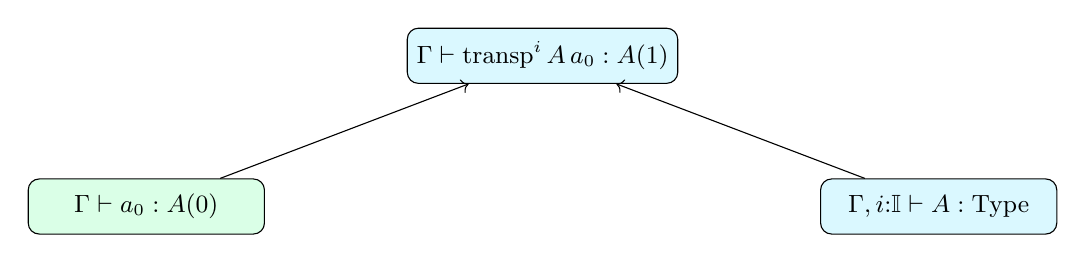
\begin{tikzpicture}[
  node distance=1.2cm and 1.8cm,
  every node/.style={font=\small},
  rule/.style={draw,rounded corners,fill=cyan!20,minimum width=3cm,minimum height=0.7cm,align=center},
  axiom/.style={draw,rounded corners,fill=green!20,minimum width=3cm,minimum height=0.7cm,align=center},
]
  \node[rule] (root) {$\Gamma \vdash \mathrm{transp}^i\,A\,a_0 : A(1)$};
  \node[axiom,below left=of root] (a) {$\Gamma \vdash a_0 : A(0)$};
  \node[rule,below right=of root] (b) {$\Gamma,i{:}\mathbb{I} \vdash A : \mathrm{Type}$};
  \draw[->] (a) -- (root);
  \draw[->] (b) -- (root);
\end{tikzpicture}
\end{center}

\noindent Each node has two visual states:
\begin{itemize}
  \item \textbf{Default:} dim gray border, term in KaTeX.
  \item \textbf{Highlighted:} colored border + glow, matching the 3D scene's
    hover color for the corresponding sub-term.
\end{itemize}

\subsection{Bidirectional Hover}

Hovering a node in the proof tree highlights the corresponding object in the
3D scene (using the existing \texttt{hoverState} store), and vice versa.
This uses the same \texttt{termKey} string already defined in each rule's
\texttt{termMappings}.

\subsection{Example: Transport Rule Proof Tree}

\[
\dfrac{
  \dfrac{}{\Gamma,\,i{:}\mathbb{I} \vdash A : \mathrm{Type}}
  \quad
  \dfrac{}{\Gamma \vdash a_0 : A(i_0)}
}{
  \Gamma \vdash \mathrm{transp}^i\,A\,[\varphi \mapsto u]\,a_0 : A(i_1)
}\ \text{(transp)}
\]

The tree collapses compound hypotheses into expandable ``...'' nodes to avoid
overflow. Clicking a node expands its sub-derivation.

\subsection{Implementation Notes}

\begin{itemize}
  \item New Svelte component: \texttt{src/lib/ProofPanel.svelte}
  \item Each \texttt{RuleDefinition} gains an optional \texttt{proofTree} field
    of type \texttt{ProofNode}:
\begin{verbatim}
interface ProofNode {
  judgment: string;     // KaTeX string
  ruleName?: string;    // label shown on the line, e.g. "transp"
  termKey?: string;     // links to 3D hover highlight
  children: ProofNode[];
}
\end{verbatim}
  \item Rendered as recursive SVG: each node is a \texttt{<foreignObject>}
    containing KaTeX; edges are \texttt{<line>} elements.
  \item Horizontal rule bar drawn between children and conclusion, labeled with
    \texttt{ruleName}.
\end{itemize}

% ─────────────────────────────────────────────────────────────────────────────
\section{Higher-Dimensional Paths: Square and Cube as Typed Terms}

\subsection{Motivation}

The primitives sidebar already has ``Square'' and ``Cube'' entries with
placeholder scenes. This feature fills them in with conceptually accurate
visualizations: a \emph{square} is a 2-dimensional path (a path-of-paths), and
a \emph{cube} is a 3-dimensional path.

These visualizations are the geometric heart of cubical type theory: every
higher homotopy is literally a higher-dimensional cube.

\subsection{Square as a Typed Term}

\paragraph{Typing rule.}
A square is a term $s : \mathrm{Sq}(A,p,q,r,t)$ where:
\[
  s : \prod_{i,j:\mathbb{I}} A \quad \text{with boundary}
  \begin{cases}
    s(i,0) = p(i) & \text{bottom face} \\
    s(i,1) = q(i) & \text{top face} \\
    s(0,j) = r(j) & \text{left face} \\
    s(1,j) = t(j) & \text{right face}
  \end{cases}
\]

\paragraph{3D visualization.}
The scene shows a filled square with four colored boundary paths:
\begin{itemize}
  \item Bottom edge $p$: \textcolor{cyan}{\textbf{cyan}} (\texttt{INTERVAL})
  \item Top edge $q$: \textcolor{orange}{\textbf{orange}} (\texttt{RESULT})
  \item Left edge $r$: \textcolor{green}{\textbf{green}} (\texttt{PARTIAL\_DATA})
  \item Right edge $t$: \textcolor{yellow}{\textbf{yellow}} (\texttt{BASE\_POINT})
  \item Interior mesh: dim translucent \textcolor{pink}{\textbf{pink}}
    (\texttt{FILL\_RESULT}, opacity 0.25)
\end{itemize}

\noindent The animation sweeps a horizontal scan line from $j=0$ to $j=1$,
tracing how $s(-,j)$ evolves from path $p$ to path $q$.

\paragraph{Steps.}
\begin{enumerate}
  \item \textbf{Boundary paths}: Display the four colored edges. Step panel
    explains that these are the four faces of the 2-cube.
  \item \textbf{Interior sweep}: Animate the scan line. Explain that $s$ is a
    homotopy from $p$ to $q$ relative to fixed endpoints.
  \item \textbf{Full square}: Show the filled mesh. Explain that the square
    itself is a term of type $A$ indexed by $\mathbb{I}^2$.
\end{enumerate}

\subsection{Cube as a Typed Term}

\paragraph{Typing rule.}
A 3-cube is a term $c : \prod_{i,j,k:\mathbb{I}} A$ with six square faces.
The faces are indexed by setting each of $i,j,k$ to $0$ or $1$.

\paragraph{3D visualization.}
The scene shows a wire-frame cube (like the Kan Filling scene but fully closed)
with face colors:
\begin{itemize}
  \item Each of the 6 faces is a distinct translucent color, one per face name.
  \item Edges shared between faces are drawn in a neutral gray.
  \item A small labeled sphere floats at the interior center labeled ``$c(i,j,k)$''.
\end{itemize}

\noindent The animation rotates the cube slowly around the $j$-axis, pausing at
each of the six face views to highlight that face and display its boundary
constraint in the step panel.

\paragraph{Steps.}
\begin{enumerate}
  \item \textbf{Three dimensions}: Show the cube skeleton and explain that
    $i,j,k : \mathbb{I}$ each range over the interval.
  \item \textbf{Six faces}: Rotate to each face in sequence; highlight the face
    and show its typing constraint.
  \item \textbf{Interior term}: Animate a point traveling through the interior,
    representing $c(i,j,k)$ for varying $i,j,k$.
\end{enumerate}

\subsection{Implementation Notes}

\begin{itemize}
  \item \texttt{src/lib/primitives/Square.svelte} and \texttt{Cube.svelte}
    (already stubbed; fill in \texttt{setup}/\texttt{update}).
  \item Square interior: \texttt{PlaneGeometry} with
    \texttt{MeshBasicMaterial(\{color, transparent, opacity: 0.25\})}.
  \item Scan line: a thin \texttt{LineSegments} object at $y = \mathrm{lerp}(0,
    2, t)$, updated each frame.
  \item Cube faces: 6 \texttt{PlaneGeometry} meshes, each slightly inset from
    the cube face to avoid z-fighting with the wireframe edges.
\end{itemize}

% ─────────────────────────────────────────────────────────────────────────────
\section{The Face Lattice $\mathbb{F}$}

\subsection{Motivation}

The face lattice $\mathbb{F}$ is the algebraic structure that governs which
faces of a cube are ``active'' in a partial element. A partial element
$[{\varphi \mapsto u}]$ is defined on exactly those points satisfying the
\emph{face formula} $\varphi \in \mathbb{F}$. Understanding $\mathbb{F}$
demystifies the notation $[\varphi \mapsto u]$ that appears in every
\texttt{comp}, \texttt{fill}, and \texttt{transp} rule.

\subsection{What is the Face Lattice?}

$\mathbb{F}$ is the free distributive lattice on generators
$\{(i=0), (i=1) \mid i \in \mathrm{Var}\}$ with the relation $(i=0)\wedge(i=1)=\bot$.
Elements of $\mathbb{F}$ are disjunctions of conjunctions of face constraints.

\paragraph{Examples (1-cube).}
\begin{align*}
  \bot &= \text{no face (empty)} \\
  (i=0) &= \text{left endpoint} \\
  (i=1) &= \text{right endpoint} \\
  (i=0)\vee(i=1) &= \text{both endpoints} \\
  \top &= \text{everywhere}
\end{align*}

\paragraph{Examples (2-cube).}
The 2-cube $\mathbb{I}^2$ has face lattice elements including:
$(i=0)$, $(j=0)$, $(i=0)\wedge(j=0)$, $(i=0)\vee(j=0)$, etc.

\subsection{Visualization: Hasse Diagram}

The primary visualization is a \textbf{Hasse diagram} of the face lattice for
the 2-cube (16 elements), drawn as an SVG or a Three.js scene with nodes and
edges.

\begin{center}
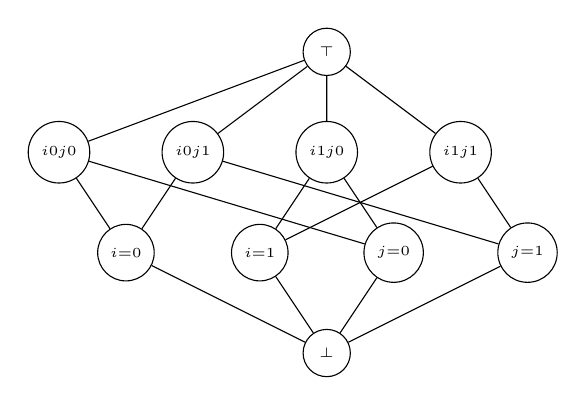
\begin{tikzpicture}[
  scale=0.85,
  node/.style={draw,circle,fill=white,minimum size=0.6cm,font=\tiny},
  >=Stealth
]
% Row 0 (bottom): bot
\node[node] (bot) at (4,0) {$\bot$};
% Row 1: four atomic faces
\node[node] (i0) at (1,1.5) {$i{=}0$};
\node[node] (i1) at (3,1.5) {$i{=}1$};
\node[node] (j0) at (5,1.5) {$j{=}0$};
\node[node] (j1) at (7,1.5) {$j{=}1$};
% Row 2: four conjunctions and four disjunctions (partial)
\node[node] (i0j0) at (0,3) {$i0j0$};
\node[node] (i0j1) at (2,3) {$i0j1$};
\node[node] (i1j0) at (4,3) {$i1j0$};
\node[node] (i1j1) at (6,3) {$i1j1$};
% Row 3 (top): top
\node[node] (top) at (4,4.5) {$\top$};
% Edges (simplified)
\draw (bot) -- (i0); \draw (bot) -- (i1); \draw (bot) -- (j0); \draw (bot) -- (j1);
\draw (i0) -- (i0j0); \draw (i0) -- (i0j1);
\draw (i1) -- (i1j0); \draw (i1) -- (i1j1);
\draw (j0) -- (i0j0); \draw (j0) -- (i1j0);
\draw (j1) -- (i0j1); \draw (j1) -- (i1j1);
\draw (i0j0) -- (top); \draw (i0j1) -- (top);
\draw (i1j0) -- (top); \draw (i1j1) -- (top);
\end{tikzpicture}
\end{center}

\noindent Node colors:
\begin{itemize}
  \item $\bot$: black
  \item $\top$: \textcolor{pink}{\textbf{pink}} (\texttt{FILL\_RESULT})
  \item Atomic faces $(i=0)$ etc.: \textcolor{green}{\textbf{green}} (\texttt{PARTIAL\_DATA})
  \item Conjunctions: \textcolor{cyan}{\textbf{cyan}} (\texttt{INTERVAL})
  \item Disjunctions: \textcolor{yellow}{\textbf{yellow}} (\texttt{BASE\_POINT})
\end{itemize}

\subsection{Interactive Mode}

Clicking a node in the Hasse diagram highlights it and:
\begin{enumerate}
  \item Displays the formula in the panel (e.g.\ ``$(i=0) \vee (j=0)$'').
  \item Shows a small 2D unit square $[0,1]^2$ with the \emph{active region}
    of that formula colored in — visually demonstrating which subset of the
    cube this formula selects.
  \item If the selected formula matches one used in another rule page (e.g.\ the
    Kan Filling rule uses $(i=0)\vee(i=1)\vee(j=0)$), a ``See in context'' link
    appears to jump to that rule.
\end{enumerate}

\subsection{Dimension Selector}

A small toggle at the top selects the dimension: \textbf{1-cube}
(5 elements, trivial), \textbf{2-cube} (16 elements, default), or
\textbf{3-cube} (too large to display fully; show a summarized view with
collapsible subtrees).

\subsection{Implementation Notes}

\begin{itemize}
  \item New page: \texttt{src/lib/FaceLattice.svelte}
  \item New route entry \texttt{'face-lattice'} in \texttt{types.ts} under
    a new sidebar category \textbf{Theory} (between Operations and Typing Rules).
  \item SVG-based layout: use a hand-rolled Sugiyama-style layered layout
    (since the lattice has a natural layer structure by rank), or adapt
    \texttt{d3-dag} if available via CDN.
  \item The 2D active-region preview uses an HTML Canvas element (100×100px)
    drawn next to the Hasse diagram.
  \item No Three.js needed for this page.
\end{itemize}

% ─────────────────────────────────────────────────────────────────────────────
\section{Univalence Proof Walkthrough}

\subsection{Motivation}

The Univalence Axiom states that equivalent types are equal:
\[
  \mathrm{ua} : (A \simeq B) \to (A =_{\mathrm{Type}} B)
\]

In cubical type theory, this is not an axiom but a \emph{theorem}, proved using
Glue types. The proof is a flagship construction that uses almost every feature
of the system: paths, transport, Kan filling, and Glue types. A multi-step
walkthrough of this proof is the most ambitious visualization in the project
and serves as a capstone for students who have worked through all other pages.

\subsection{Structure of the Proof}

The proof has four stages:

\begin{enumerate}
  \item \textbf{Setup}: Given $e : A \simeq B$, define a line of types
    $\mathrm{Glue}\,[\,i=0 \mapsto (A,e),\;i=1 \mapsto (B,\mathrm{id})\,]$.
  \item \textbf{Glue construction}: Show that this Glue type at $i=0$ is
    definitionally $A$ and at $i=1$ is definitionally $B$.
  \item \textbf{Path in the universe}: The line of Glue types gives a path
    $i \mapsto \mathrm{GlueType}(i)$ in $\mathrm{Type}$, which is exactly
    $A =_{\mathrm{Type}} B$.
  \item \textbf{Corollary}: Transport along this path gives the underlying
    function of $e$, closing the loop.
\end{enumerate}

\subsection{Multi-Page Walkthrough Design}

This feature is implemented as a \textbf{multi-page guided tour} rather than
a single rule page. A persistent top bar displays a progress indicator:

\begin{center}
\texttt{[ Setup ] → [ Glue ] → [ Path in Type ] → [ Transport ] }
\end{center}

\noindent Each stage is a full-page view with:
\begin{itemize}
  \item A 3D scene (reusing and composing existing rule scenes).
  \item An annotation layer: arrows and labels overlaid on the 3D canvas
    pointing to specific objects with explanatory callouts.
  \item A text panel on the right with the proof fragment in KaTeX.
\end{itemize}

\subsection{Scene Designs Per Stage}

\paragraph{Stage 1: Setup.}
Show two spheres labeled $A$ and $B$ connected by a labeled arc $e$
(like the Glue Types scene). A faint dotted line appears between them
labeled $i \in [0,1]$, previewing the path about to be constructed.
Color $A$ in \textcolor{cyan}{\textbf{cyan}}, $B$ in \textcolor{orange}{\textbf{orange}}.

\paragraph{Stage 2: Glue Construction.}
Morph the previous scene: the arc $e$ thickens into a cylinder representing
the Glue type. Small text sprites on the cylinder ends read
``$\mathrm{Glue}(0) = A$'' and ``$\mathrm{Glue}(1) = B$''. A cross-section
slider lets the user drag $i \in [0,1]$ to inspect $\mathrm{Glue}(i)$.

\paragraph{Stage 3: Path in the Universe.}
Zoom out to show ``$\mathrm{Type}$'' as a large ambient space (dark background,
subtle grid). The cylinder from Stage 2 appears as a curved path in this space
from $A$ to $B$. Label the path ``$A =_\mathrm{Type} B$''.

\paragraph{Stage 4: Transport.}
Split-screen: left shows the path in Type; right shows a point $a : A$
being transported along the path, arriving as $e(a) : B$.
This reuses the TransportRule scene with appropriate labels.

\subsection{Interaction}

\begin{itemize}
  \item \textbf{Stage navigation}: Prev/Next buttons in the top bar.
  \item \textbf{Within each stage}: the standard step panel from other rules.
  \item \textbf{Cross-links}: ``Review: Glue Types'', ``Review: Transport''
    buttons link to the corresponding rule pages.
  \item \textbf{Completion}: On finishing Stage 4, a congratulations message
    and a summary proof in a modal window.
\end{itemize}

\subsection{Implementation Notes}

\begin{itemize}
  \item New top-level route: \texttt{'univalence'} in \texttt{types.ts}.
  \item New component: \texttt{src/lib/Univalence.svelte} — manages the
    stage state and renders each stage's sub-component.
  \item Sub-components: \texttt{UniSetup.svelte}, \texttt{UniGlue.svelte},
    \texttt{UniPath.svelte}, \texttt{UniTransport.svelte}.
  \item Stage 3 ambient space: large \texttt{PlaneGeometry} grid
    at $y = -5$ with \texttt{GridHelper}; camera pulled back to
    $z = 20$.
  \item The annotation layer is an absolutely positioned \texttt{<svg>}
    overlaid on the Three.js canvas, using projected 3D coordinates:
    \texttt{vector.project(camera)} converts world coords to clip space
    for overlay positioning.
\end{itemize}

% ─────────────────────────────────────────────────────────────────────────────
\section{Dependency Graph Navigation}

\subsection{Motivation}

The current sidebar is a flat list of categories. As the number of rule pages
grows, students need a way to see \emph{how concepts build on each other}.
Which rules depend on the interval? Which rules use Glue types? The
\emph{Dependency Graph} provides a bird's-eye view of the system's structure
and serves as an alternative navigation surface.

\subsection{Graph Structure}

Nodes are all pages in \texttt{cubical-viz}. Directed edges go from
\emph{dependency} to \emph{dependent}: an edge $A \to B$ means ``rule $B$
uses concept $A$''. The graph for the current set of pages is:

\begin{center}
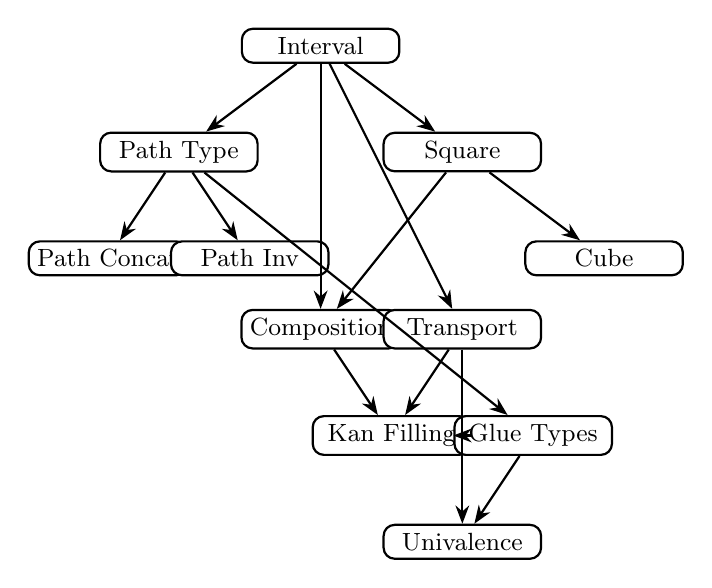
\begin{tikzpicture}[
  scale=0.9,
  node/.style={draw,rounded corners,fill=white,font=\small,minimum width=2cm,align=center,inner sep=3pt},
  >=Stealth,thick
]
\node[node] (I)   at (0,4)    {Interval};
\node[node] (PT)  at (-2,2.5) {Path Type};
\node[node] (Sq)  at (2,2.5)  {Square};
\node[node] (Cu)  at (4,1)    {Cube};
\node[node] (PC)  at (-3,1)   {Path Concat};
\node[node] (PI)  at (-1,1)   {Path Inv};
\node[node] (Co)  at (0,0)    {Composition};
\node[node] (Tr)  at (2,0)    {Transport};
\node[node] (KF)  at (1,-1.5) {Kan Filling};
\node[node] (GT)  at (3,-1.5) {Glue Types};
\node[node] (UA)  at (2,-3)   {Univalence};
\draw[->] (I) -- (PT); \draw[->] (I) -- (Sq); \draw[->] (Sq) -- (Cu);
\draw[->] (PT) -- (PC); \draw[->] (PT) -- (PI);
\draw[->] (I) -- (Co); \draw[->] (I) -- (Tr);
\draw[->] (Sq) -- (Co); \draw[->] (Co) -- (KF); \draw[->] (Tr) -- (KF);
\draw[->] (KF) -- (GT); \draw[->] (PT) -- (GT);
\draw[->] (GT) -- (UA); \draw[->] (Tr) -- (UA);
\end{tikzpicture}
\end{center}

\subsection{Visual Design}

\paragraph{Layout.}
The graph is laid out using a \emph{force-directed layout} (via a minimal
D3-force simulation or a hand-rolled Fruchterman–Reingold iteration).
Alternatively, since the graph is a DAG, a Sugiyama layered layout cleanly
separates the levels (Interval at top, Univalence at bottom).

\paragraph{Nodes.}
Each node is a rounded rectangle with:
\begin{itemize}
  \item The rule icon (same as sidebar).
  \item The rule name.
  \item A small color dot matching the rule's primary color in the 3D scene.
  \item Hover: a tooltip with the rule's one-sentence description.
\end{itemize}

\noindent Completed pages are shown in full color; pages not yet implemented
are shown in gray with a ``coming soon'' badge.

\paragraph{Edges.}
Directed edges with arrowheads. Color: \texttt{rgba(255,255,255,0.25)} (dim
white). On hover over a node, all edges to/from that node brighten to full
white and direct dependencies are highlighted in \textcolor{cyan}{\textbf{cyan}}
while dependents are highlighted in \textcolor{orange}{\textbf{orange}}.

\paragraph{Background.}
Dark background (\texttt{\#0d1117}), subtle dot-grid pattern.

\subsection{Interaction}

\begin{itemize}
  \item \textbf{Click node}: Navigate to that rule page (equivalent to clicking
    the sidebar entry).
  \item \textbf{Hover node}: Show dependency highlights and tooltip.
  \item \textbf{Pan and zoom}: Mouse drag to pan; scroll wheel to zoom (via
    D3 zoom or custom transform).
  \item \textbf{Keyboard}: \texttt{/} focuses a search box that filters nodes
    by name.
  \item \textbf{``Show all paths to X''}: Right-click a node to highlight all
    transitive dependency paths leading to it, showing the ``learning path'' to
    that concept.
\end{itemize}

\subsection{Access}

The dependency graph is accessible via:
\begin{enumerate}
  \item A new sidebar entry at the very top: \textbf{Overview} with a graph icon.
  \item A ``View in graph'' link at the top of every rule page.
  \item URL: \texttt{\#overview} or \texttt{\#graph}.
\end{enumerate}

\subsection{Implementation Notes}

\begin{itemize}
  \item New component: \texttt{src/lib/DependencyGraph.svelte}.
  \item New entry \texttt{'overview'} in \texttt{types.ts} under a new category
    \textbf{Overview} at the top of the sidebar.
  \item SVG-based rendering (not Three.js) for the graph itself.
  \item Dependency data: a static \texttt{DEPS} map in \texttt{types.ts}:
\begin{verbatim}
const DEPS: Partial<Record<VisualizationType,
                           VisualizationType[]>> = {
  'path-type-rule':    ['interval'],
  'square':            ['interval'],
  'composition-rule':  ['interval', 'square'],
  ...
};
\end{verbatim}
  \item Force layout: 200 iterations of Fruchterman–Reingold on mount,
    then frozen (no continuous simulation to avoid battery drain).
\end{itemize}

% ─────────────────────────────────────────────────────────────────────────────
\section{Priority and Sequencing}

Table~\ref{tab:priority} gives a suggested implementation order based on
difficulty and pedagogical value.

\begin{table}[h]
\centering
\begin{tabular}{lllp{5cm}}
\toprule
\textbf{Order} & \textbf{Feature} & \textbf{Effort} & \textbf{Rationale} \\
\midrule
1 & Square / Cube (Sec.~3) & Medium & Fills existing stubs; high visual impact \\
2 & Dependency Graph (Sec.~6) & Medium & Improves navigation for all existing pages \\
3 & Face Lattice $\mathbb{F}$ (Sec.~4) & Medium & Unlocks understanding of partial elements \\
4 & Proof Relevance Panel (Sec.~2) & Medium–Hard & Adds depth to all existing rules \\
5 & Univalence Walkthrough (Sec.~5) & Hard & Flagship capstone; requires all others \\
\bottomrule
\end{tabular}
\caption{Suggested implementation order.}
\label{tab:priority}
\end{table}

% ─────────────────────────────────────────────────────────────────────────────
\section{Conclusion}

These five features complete the pedagogical arc of \texttt{cubical-viz}: from
individual rules (Phase 1--2) to a fully connected, navigable, proof-aware
learning environment. The most immediately impactful additions are the
Square/Cube visualizations (filling existing stubs) and the Dependency Graph
(making the system navigable as it grows). The Univalence Walkthrough serves
as the capstone that ties everything together.

\end{document}
